\documentclass[12pt,letterpaper]{article}
\usepackage{amsmath,amssymb}
\usepackage[margin=1in]{geometry}
\usepackage{enumitem}
\usepackage{tikz}
\usetikzlibrary{arrows.meta,decorations.markings}
\tikzset{
  boundary/.style={line width=0.9pt,postaction={decorate},
    decoration={markings,mark=at position 0.6 with {\arrow{Stealth}}}},
  regionaxis/.style={gray,thin,-{Stealth[length=4pt]}},
  every picture/.style={font=\footnotesize}
}

\setlength{\parindent}{0pt}
\setlength{\parskip}{4pt}

\begin{document}

\textbf{MATH 261, Homework Set 7 --- Answers}

\small
\setlength{\abovedisplayskip}{6pt}
\setlength{\belowdisplayskip}{6pt}
\setlength{\abovedisplayshortskip}{3pt}
\setlength{\belowdisplayshortskip}{6pt}

\begin{enumerate}[leftmargin=*,itemsep=2pt,parsep=0pt,topsep=6pt]
\item $\nabla\cdot\mathbf F=4y$; curl $k$-component $=0$; conservative: yes.
\item $\nabla\cdot\mathbf F=2x\cos(x^2)+2ye^{y^2}$;
      curl $k$-component $=1$; conservative: no.
\item $\nabla\cdot\mathbf F=2x$;
      $\nabla\times\mathbf F=(x-2z,-y,0)$; conservative: no.
\item $\nabla\cdot\mathbf F=0$;
      $\nabla\times\mathbf F=(0,-3x^2,0)$; conservative: no.
\item $\nabla\cdot\mathbf F=0$;
      $\nabla\times\mathbf F=(0,0,0)$; conservative: yes.
\item $\nabla\cdot\mathbf F=-xz\cos y$;
      $\nabla\times\mathbf F=(0,0,0)$; conservative: yes.
\item At $(1,-1,1)$: curl $=(2,0,0)$; divergence $=7$.
\item At $(1,-1,1)$: curl $=(0,3,4)$; divergence $=-9$.
\item $f=x^2+3y+2z^2+C$.
\item $f=xy^2+ye^z+C$.
\item $f=x\cos z+y^2+C$.
\item $16$.
\item $0$.
\item Direct line integral: $2\pi$; Green's theorem: $2\pi$.
\item Direct line integral: $0$; Green's theorem: $0$.
\item $\dfrac12$.
\item $\dfrac76$.
\item $3(26-e^5)$.
\item $\dfrac92(e^5+9)$.
\item $-1$.
\item $-\dfrac13$.
\item $-\dfrac5{12}$.
\item $-\dfrac13$.
\item $0$.
\item $\dfrac{22}{15}$.
\end{enumerate}

\newpage
\textbf{Worked solutions: Problems 7, 21, and 23}

\medskip
\textbf{7. Curl and divergence at $(1,-1,1)$.}

Write $\mathbf F=(P,Q,R)=(x^2z,-2y^2z^2,xy^2z)$. Then
\[
\begin{aligned}
\nabla\cdot\mathbf F
  &=P_x+Q_y+R_z=2xz-4yz^2+xy^2,\\
(\nabla\cdot\mathbf F)(1,-1,1)
  &=2+4+1=\boxed{7}.
\end{aligned}
\]
The curl is
\[
\begin{aligned}
\nabla\times\mathbf F
  &=(R_y-Q_z,\ P_z-R_x,\ Q_x-P_y)\\
  &=(2xyz-(-4y^2z),\ x^2-y^2z,\ 0-0),\\
(\nabla\times\mathbf F)(1,-1,1)
  &=(-2+4,\ 1-1,\ 0)=\boxed{(2,0,0)}.
\end{aligned}
\]

\medskip
\textbf{21. Outward flux across the triangle from Problem 20.}

\noindent\begin{minipage}[c]{0.56\linewidth}
\raggedright
Here $\mathbf F=(P,Q)=(x^2+y,y^2-x)$.
The shaded triangle $D$ has bounds
\[
\left\{
\begin{aligned}
&-1\leq x\leq0,\\
&0\leq y\leq-x.
\end{aligned}
\right.
\]
\end{minipage}\hfill
\begin{minipage}[c]{0.40\linewidth}
\centering
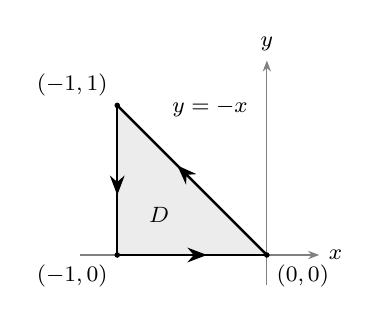
\begin{tikzpicture}[x=1.9cm,y=1.9cm]
  \fill[gray!15] (-1,0)--(0,0)--(-1,1)--cycle;
  \draw[regionaxis] (-1.25,0)--(0.35,0) node[right,black] {$x$};
  \draw[regionaxis] (0,-0.2)--(0,1.3) node[above,black] {$y$};
  \draw[boundary] (-1,0)--(0,0);
  \draw[boundary] (0,0)--(-1,1);
  \draw[boundary] (-1,1)--(-1,0);
  \fill (-1,0) circle (1pt) node[below left] {$(-1,0)$};
  \fill (0,0) circle (1pt) node[below right] {$(0,0)$};
  \fill (-1,1) circle (1pt) node[above left] {$(-1,1)$};
  \node at (-0.38,0.98) {$y=-x$};
  \node at (-0.72,0.27) {$D$};
\end{tikzpicture}
\end{minipage}

For the outward unit normal $\mathbf N$, Green's flux formula uses
$P_x+Q_y=2x+2y$. Thus
\[
\begin{aligned}
\oint_C\mathbf F\cdot\mathbf N\,ds
 &=\iint_D(P_x+Q_y)\,dA
   =\int_{-1}^0\int_0^{-x}(2x+2y)\,dy\,dx\\
 &=\int_{-1}^0[2xy+y^2]_0^{-x}\,dx
   =\int_{-1}^0-x^2\,dx
   =\left[-\frac{x^3}{3}\right]_{-1}^0
   =\boxed{-\frac13}.
\end{aligned}
\]
\medskip
\textbf{23. Work around the triangle between $y=-x$ and $y=x$.}

\noindent\begin{minipage}[c]{0.56\linewidth}
\raggedright
The traversal
$(0,0)\to(1,-1)\to(1,1)\to(0,0)$ is counterclockwise.
The shaded region $D$ has bounds
\[
\left\{
\begin{aligned}
&0\leq x\leq1,\\
&-x\leq y\leq x.
\end{aligned}
\right.
\]
\end{minipage}\hfill
\begin{minipage}[c]{0.40\linewidth}
\centering
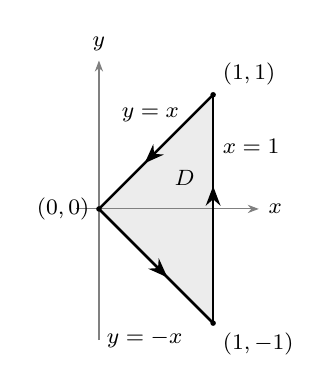
\begin{tikzpicture}[x=1.45cm,y=1.45cm]
  \fill[gray!15] (0,0)--(1,-1)--(1,1)--cycle;
  \draw[regionaxis] (-0.2,0)--(1.4,0) node[right,black] {$x$};
  \draw[regionaxis] (0,-1.15)--(0,1.3) node[above,black] {$y$};
  \draw[boundary] (0,0)--(1,-1);
  \draw[boundary] (1,-1)--(1,1);
  \draw[boundary] (1,1)--(0,0);
  \fill (0,0) circle (1pt) node[left] {$(0,0)$};
  \fill (1,-1) circle (1pt) node[below right] {$(1,-1)$};
  \fill (1,1) circle (1pt) node[above right] {$(1,1)$};
  \node at (0.45,0.82) {$y=x$};
  \node at (0.4,-1.14) {$y=-x$};
  \node[right] at (1,0.55) {$x=1$};
  \node at (0.75,0.27) {$D$};
\end{tikzpicture}
\end{minipage}

For $P=x^2y$ and $Q=xy^2$, we have $Q_x-P_y=y^2-x^2$.
Using the circulation form of Green's theorem,
\[
\begin{aligned}
W&=\oint_C P\,dx+Q\,dy
  =\int_0^1\int_{-x}^{x}(y^2-x^2)\,dy\,dx\\
 &=\int_0^1\left[\frac{y^3}{3}-x^2y\right]_{-x}^{x}\,dx
  =\int_0^1-\frac43x^3\,dx
  =\left[-\frac{x^4}{3}\right]_0^1
  =\boxed{-\frac13}.
\end{aligned}
\]
\end{document}
